\documentclass{article}
\usepackage[utf8]{inputenc}
\usepackage{graphicx}


%https://tex.stackexchange.com/a/139403
\graphicspath{{./Figures/}}
% double curly braces important!
\begin{document}

\Large{\title{\textbf{Proof of Concept}}}
\author{Bree Kelly} \date{}

\maketitle

\paragraph{} ~\\ \large
\noindent{\textbf{Elaboration I}}
\newline \break
I want to take a passage of hieroglyphic text through the process of translation, using the Hieroglyphics Initiative as a digital tool.
\newline ~\\
For example, if I were to use the platform to assist me in translating the passage below from the Story of Sinuhe:
\paragraph{}~\\
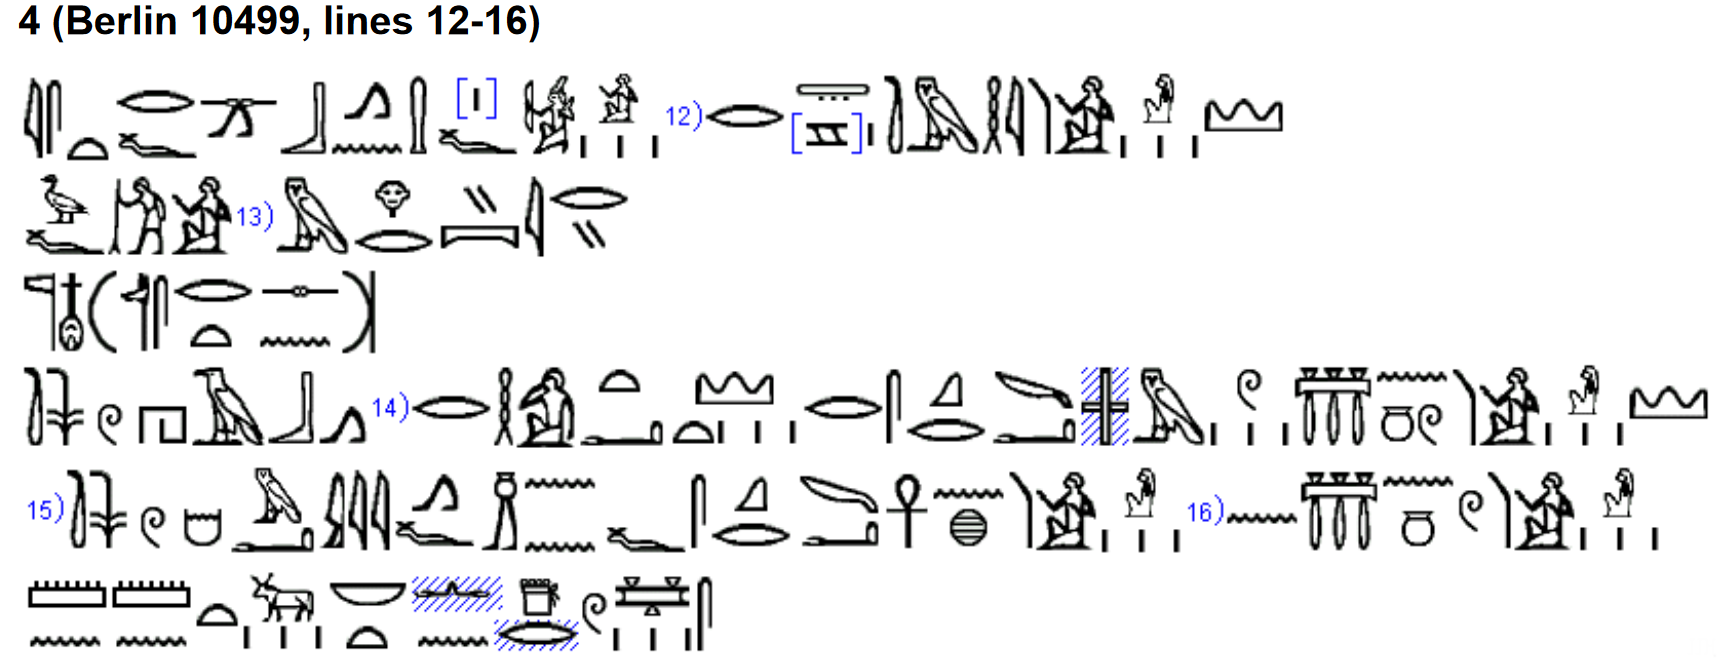
\includegraphics[width=1.0\textwidth]{hiero_1.PNG}
%http://carrington-arts.com/JJSinuhe/Sinuhe.pdf
\paragraph{}~\\
Will the tool be able to:
\newline ~\\
\begin{itemize}  
\item Generate a readable facsimile from a source image?
\item Identify individual signs correctly?
\item Identify groupings of signs correctly?
\item Provide accurate information on the meaning of these signs and groupings?
\item Provide accurate information on the potential transliteration of the text?
\end{itemize}
\paragraph{} ~\\ \noindent \textbf{Challenges:}
\newline \break \noindent
There isn't a lot of documentation on what this tool can and cannot do, so this will actually be an exercise in figuring that out.
\newline \break \noindent
Any pitfalls that the tool suffers from cannot be known yet, as it is not widely documented or available for use yet.
\newline \break \noindent
There is no way of knowing what the pitfalls and limitations of the tool are without being able to test it.
\newline \break \noindent
I will not be able to test any of these issues or steps until I gain access to the tool itself.
\newline \break \noindent
To what extent does it actually assist in the process of translating hieroglyphs?
\newline \break \noindent
What do I want it to do? Provide information along the way - be able to be interacted with in order to determine what the signs and groups of signs are, which will lead to a transliteration, then provide interactive dictionary tools to create a translation.
\newline \break \noindent
Are there examples of this being done? Not that I know of, at least not specifically using the Hieroglyphics Initiative itself. There are older programs that were used in hieroglyph translation: Glyph, WinGlyph, MacScribe, Inscribe, VisualGlyph, VectorOffice and Hieroglyphica.

%Gozzoli, R. (2013), ‘Hieroglyphic Text Processors, Manuel de Codage, Unicode, Lexicon,’ in S. Polis, and J. Winand (eds.), Technology, Texts, Languages and Information Technology in Egyptology, Selected papers from the meeting of the Computer Working Group of the International Association of Egyptologists (Informatique & Égyptologie), Presses Universitaires de Liège, Liège, 89-101. 

\newpage \noindent{\textbf{Elaboration II}}
\newline \break \noindent
In order to test the tool step by step, I took the following passage through the process of manual translation, then repeated this process using The Hieroglyphics Initiative:
\newline \break
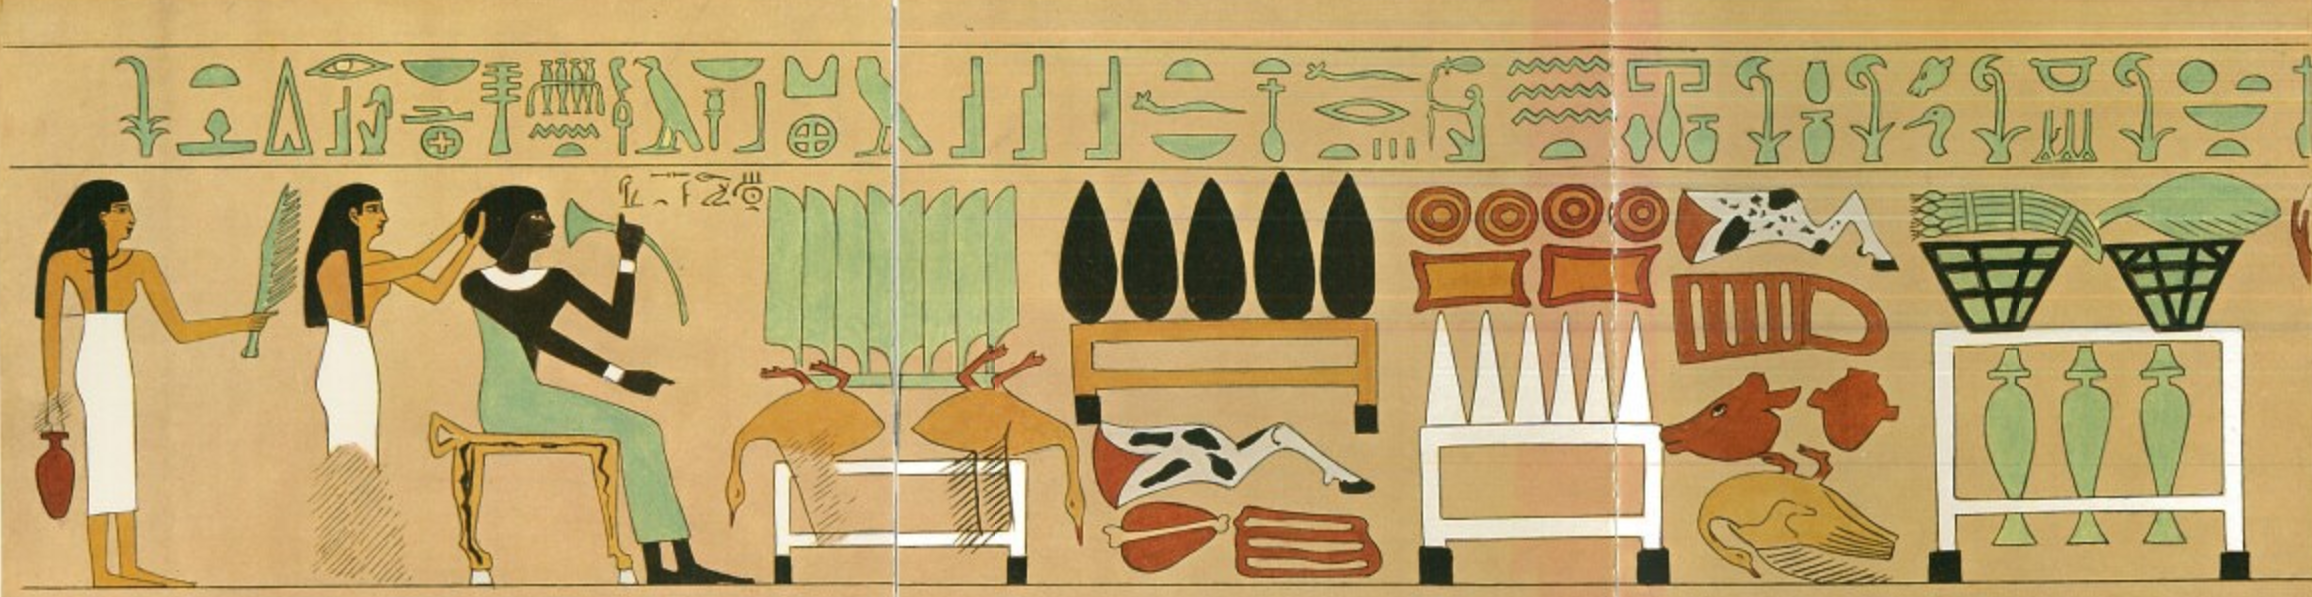
\includegraphics[width=1.0\textwidth]{hiero_2.PNG}
\break \noindent \underline{Source}: Naville, E.,\textit{ The XIth Dynasty Temple at Deir el-Bahari III}, pl. III.
%source of passage: http://meketre.org/repository/theme/1114116?fbclid=IwAR2sPwrQy0Ev1l7JfAhMEO7TH3yWER5ShsSYZYVxc-s_vHYsew1e5OmCR_8
\newline \break \noindent
\underline{Step-by-Step Process of Translation}:
\newline \break
Identify each individual sign using Gardiner's List.
\newline \break
Identify sign groupings to form words.
\newline \break
Interpret signs and sign groupings to produce transliteration.
\newline \break
Translate words in English to form phrases.
\newline \break
Using knowledge of Hieroglyphic grammar to to form sentences.
\newline \break \noindent
\underline{Step-by-Step Process using The Hieroglyphics Initiative}:
\newline \break \noindent
\underline{Step 1}: Gain access to tool (The Hieroglyphics Initiative)
\newline \break \noindent
In order to establish access to the tool so that I can experiment with it, I needed to get in contact with the developers themselves. With the help of Brian, I was added to the Slack Workspace for The Hieroglyphics Initiative, and through email correspondence with Alex Fry, the Technology Director, I was sent a link to the Workbench. At first, I still could not access it, as my email accounts had not been given permission yet, but after Brian helped me contact Alex directly through Slack, both my student email (bree.kelly@students.mq.
\newline edu.au) and staff email (bree.kelly@mq.edu.au) were approved and I could finally access the Workbench. I have been using my staff email to gain access, although both email accounts are approved (both are registered with Google now). Using the web browser Firefox, I was successful in opening the Workbench.
\newline \break \noindent
Step 1 achieved.
\newline \break \noindent
\underline{Step 2}: Upload image of hieroglyphic text.
\newline \break \noindent
For this step, I went online to find a repository of images that included hieroglyphic passages. I found a repository site called `Meket Scene Repository' (http://meketre.org/repository/search) and looked through the images available until I came across a scene from Theban Tomb 308 depicting grooming and beauty treatment of women. I could see in the preview thumbnail that there were hieroglyphs in the image. Although this image is not a photo of a wall, but a reconstruction, I thought it would make a good test image for this exercise. I saved the image as a PNG file, using the Windows Snipping Tool (the browser would not let me save the image any other way). Curious as to what files the Workbench would allow to be uploaded, I attempted to upload a .tif file. It did not like this. `Image load error.' I have established that it is okay with uploading JPG and PNG. I have to wonder about the use of JPG files, however, as they are a type of image file most prone to data loss, which might be fine when it comes to recreational use by the wider public, but in the academic domain, this is less than desirable. I brought this up to Brian and he agreed, stating that RAW is probably the most desirable file type, with cameras able to capture their images in such a file format, meaning that from the very start of the process (ie. capture of the hieroglyphic image itself), the file type would be both consistent and experience the least amount of data loss possible. I successfully uploaded my PNG file into the Workbench.
\newline \break \noindent
Step 2 achieved.
\newline \break \noindent
\underline{Note}: I tried uploading a previous project (provided in the links in the Documentation pdf from Alex's email) from the Beni Hasan folder, and it would not upload in Firefox. It would say `Upload Error'. At this point, I downloaded Chrome onto my Surface and switched to using Chrome for use of the Workbench (it makes sense that Chrome supports it best, as this is a Google project now).
\newline \break \noindent
\underline{Step 3}: 
Select passage of Hieroglyphs using Marquee tool, turn Threshold tool to `active' and adjust Threshold level.
\newline \break
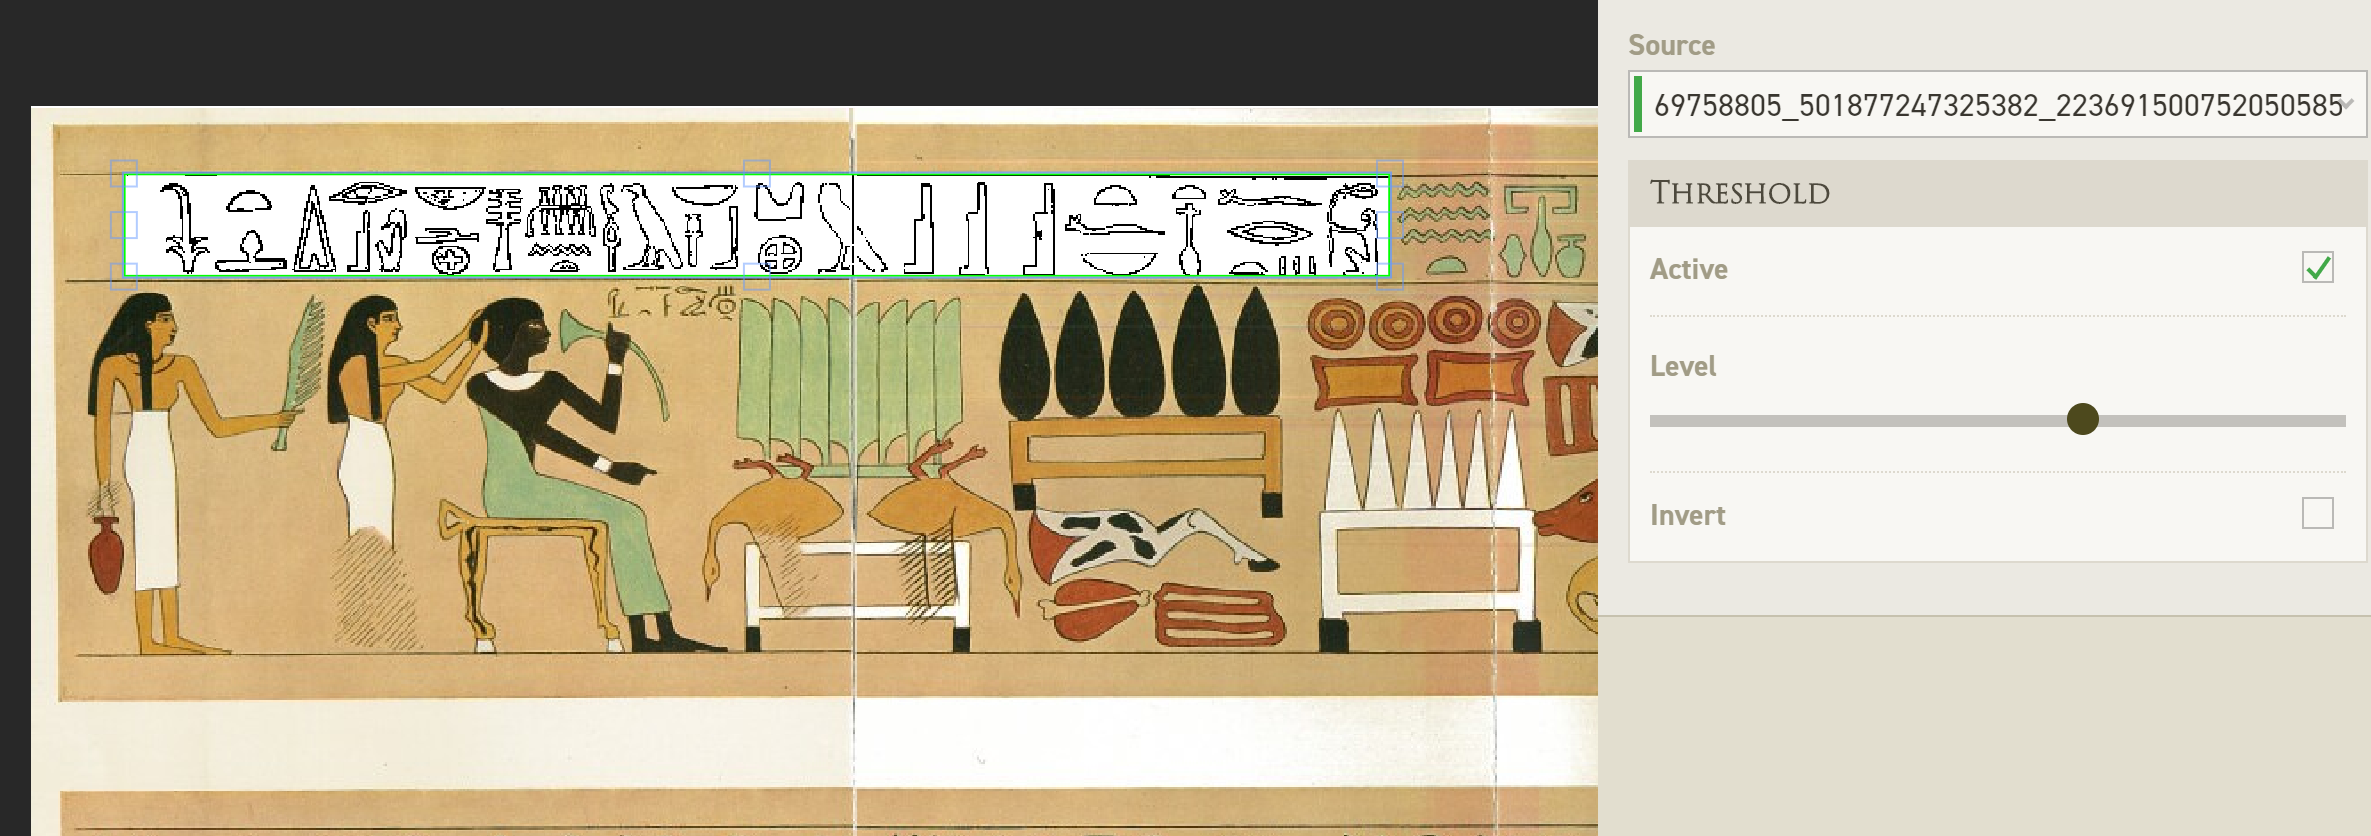
\includegraphics[width=1.0\textwidth]{hiero_3.PNG}
\break \noindent This is all done in the `1. Process' stage/tab.
\newline \break

\includegraphics[width=1.0\textwidth]{hiero_4.PNG}
\break \noindent
I successfully adjusted the threshold to the desired level, where the outlines of the hieroglyphic signs are clear and hopefully readable.
\newline \break \noindent
Step 3 achieved.
\newline \break \noindent
\underline{Note}: I tried the 'Invert' function of the threshold tool for a random image of hieroglyphics that I found on Google Images, which has dark areas near its left and right hand edges:
\newline \break
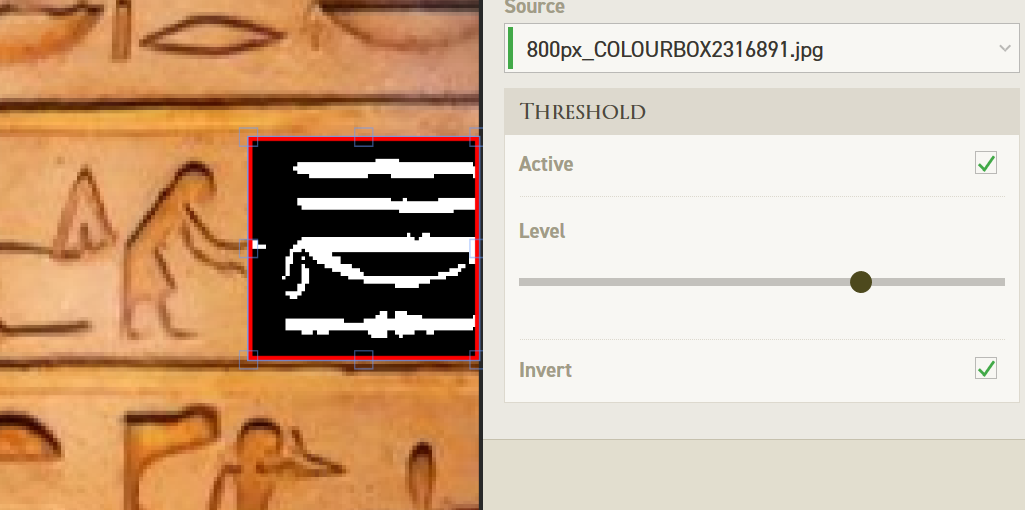
\includegraphics[width=1.0\textwidth]{hiero_5.PNG}
\newline \break \noindent
\underline{Step 4}: I am now moving onto the `2. Generate' section/tab.
\newline \break

\includegraphics[width=1.0\textwidth]{hiero_7.PNG}
\newline \break \noindent
I want to clean up the unneeded lines and imperfections in the following image:
\newline \break
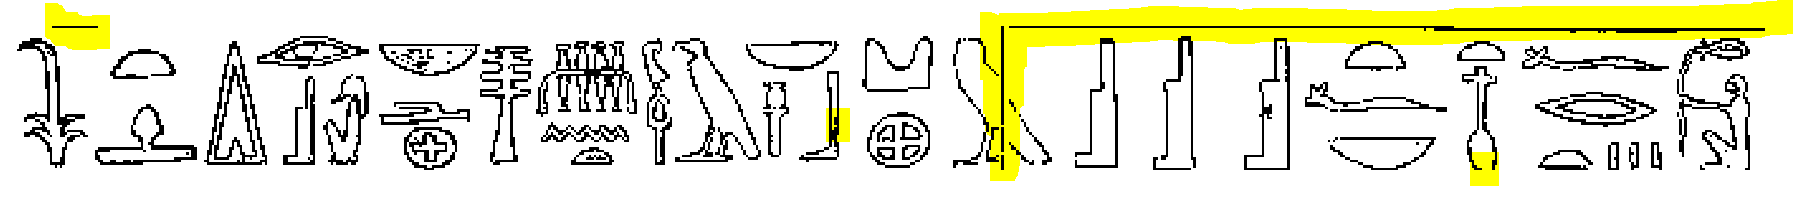
\includegraphics[width=1.0\textwidth]{hiero_8.PNG}
By making the Draw/Erase tools `active,' I use the Erase tool to remove the unneeded blemishes. I made some mistakes during this stage and the Undo and Redo tools work as expected.
\newline \break
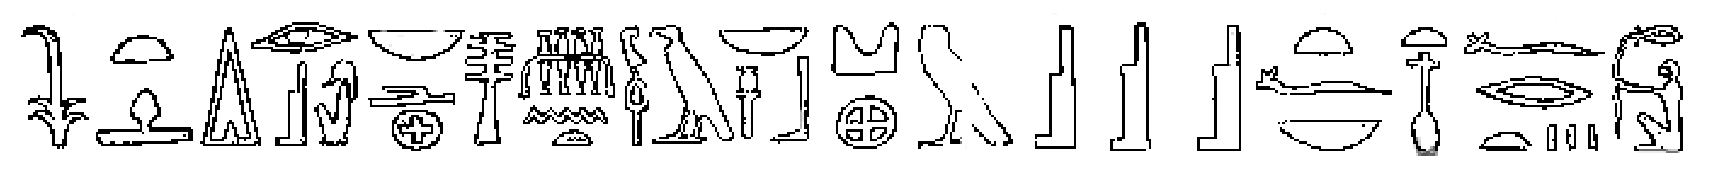
\includegraphics[width=1.0\textwidth]{hiero_9.PNG}
The Outline tool also appears to work, but I won't really use it in this example:
\newline \break
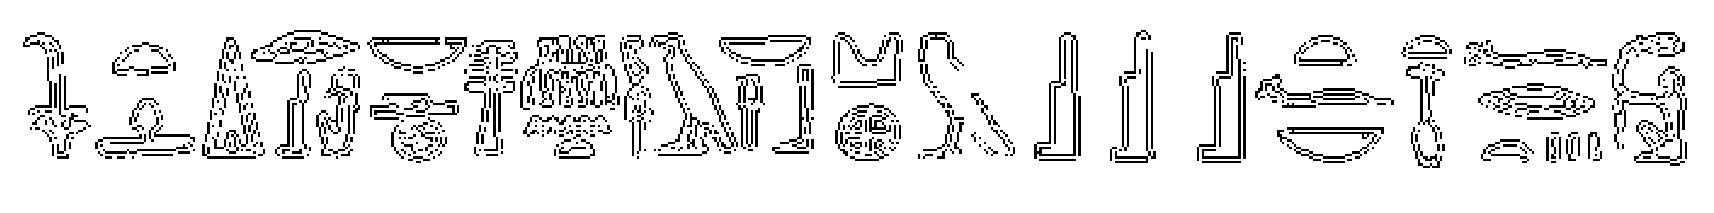
\includegraphics[width=1.0\textwidth]{hiero_10.PNG}
\break \noindent Facsimile has been touched up successfully.
\newline \break \noindent
Step 4 achieved.
\newline \break \noindent
\underline{Step 5}: Time for `3. Analyse' section/tab
\newline \break

\includegraphics[width=1.0\textwidth]{hiero_11.PNG}
\break \noindent
In this section, the aim is to analyse the signs and hopefully also some sign groupings. You have two ways of doing this - either using the Marquee tool to select a whole line or phrase, or using the Polygon tool to select an individual sign. I try out the Polygon tool first:
\newline \break
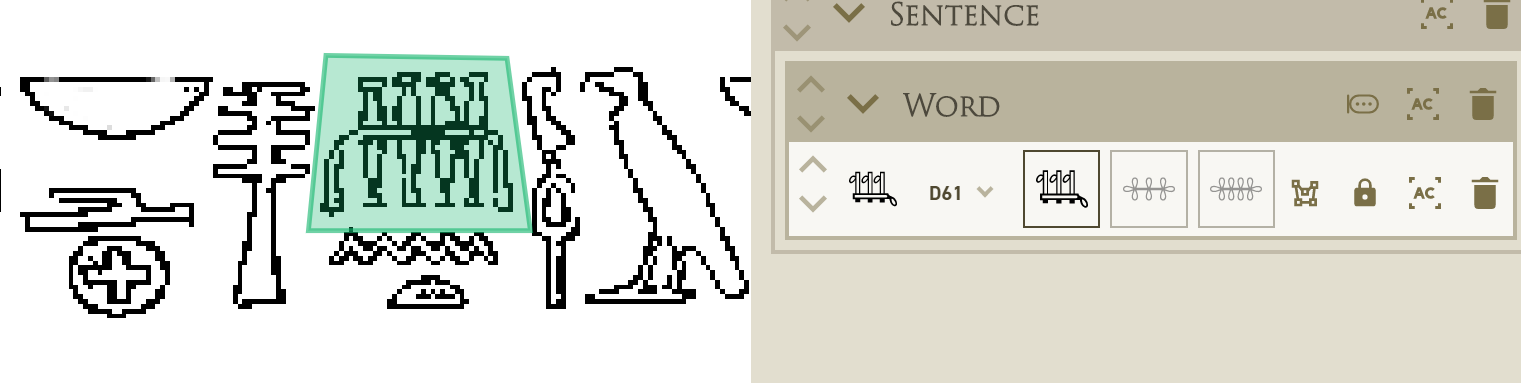
\includegraphics[width=1.0\textwidth]{hiero_12.PNG}
\break \noindent
Despite my facsimile still not being overly clear, the sign I manually selected using the Polygon tool was still able to be identified by the auto-identify.
\newline \break \noindent
However, you might notice that the sign it has been identified as isn't \textit{quite} correct. (This is where my knowledge of Hieroglyphs comes in handy). I can tell that even though the image is still quite rough, the sign I have highlighted is actually W18 from Gardiner's Sign, not D61, as the tool claims. The tool does allow me to fix this, fortunately. By clicking on the arrow next to where it says `D61,' I can select a new option, which will replace the current identification.
\newline \break
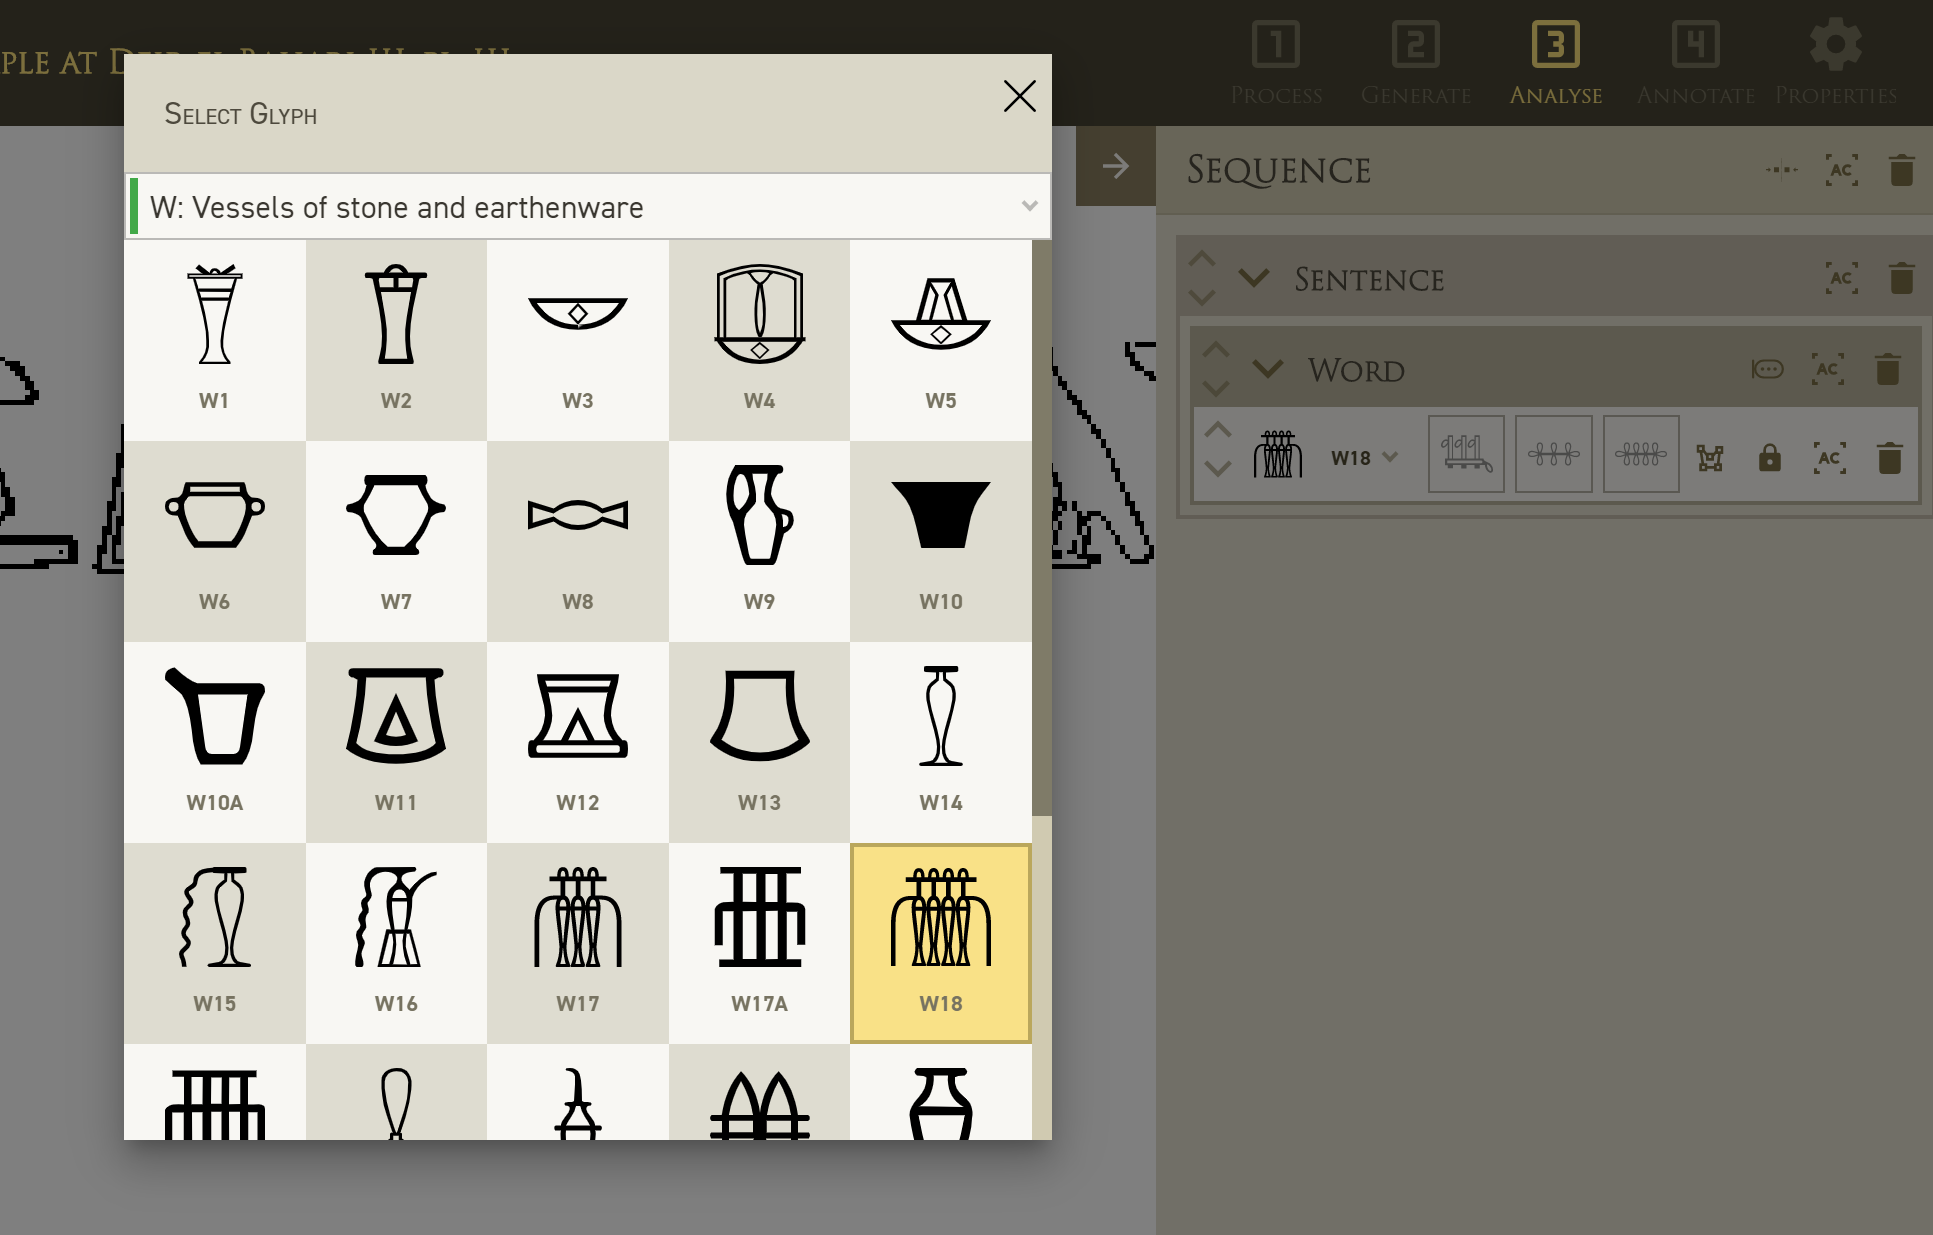
\includegraphics[width=1.0\textwidth]{hiero_13.PNG}
\break \noindent
That's better.
\newline \break \noindent
Now, to try out the Auto-Identify option using the Marquee tool. I selected my whole passage using the Marquee tool, and it appears to have identified most of the signs as signs. There is one sign that it had trouble with, being the owl, which I failed to touch up the outline of in the previous steps. It has identified this sign as three different signs, and understandably has been unable to auto-identify any of these (obviously, because they are just random shapes at this point). As the system has not been able to identify any of the signs by itself and I will need to manually classify (and potentially correct) each sign, it appears to have 
\newline \break
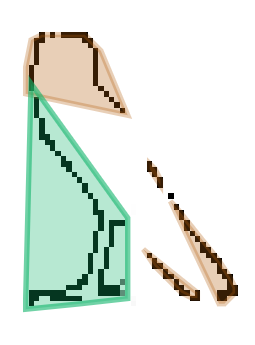
\includegraphics[width=0.2\textwidth]{hiero_14.PNG}
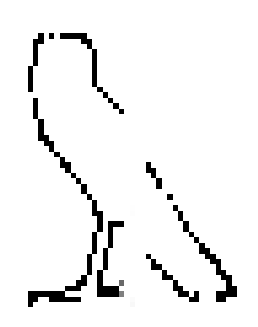
\includegraphics[width=0.2\textwidth]{hiero_15.PNG}
\break \noindent
I return to the Generate tab and fix this up using the Draw tool. I then return to the Analyse tab and delete the individual `glyphs' the Marquee/Auto-Identify tool has identified and manually select the glyph using the Polygon tool. It is now outside of the 'sentence' identified by the auto-identify (which considers all of the glyphs to form one 'word' at this stage). I use the Classify tool to let the system auto-classify the owl glyph. It interprets the owl as G36 (the so-called \textit{wr}-bird) but I easily correct this using the drop down arrow next to the G36, as in the above example.
\newline \break \noindent
Moving onto The Hieroglyphics Initiative's ability to translate - down the bottom of the window is a Translation section. Using just the first phrase (which I am treating as a 'word' for the sake of the exercise), I test out the Auto-Translate tool and also enter my own transliteration and translation.
\newline \break
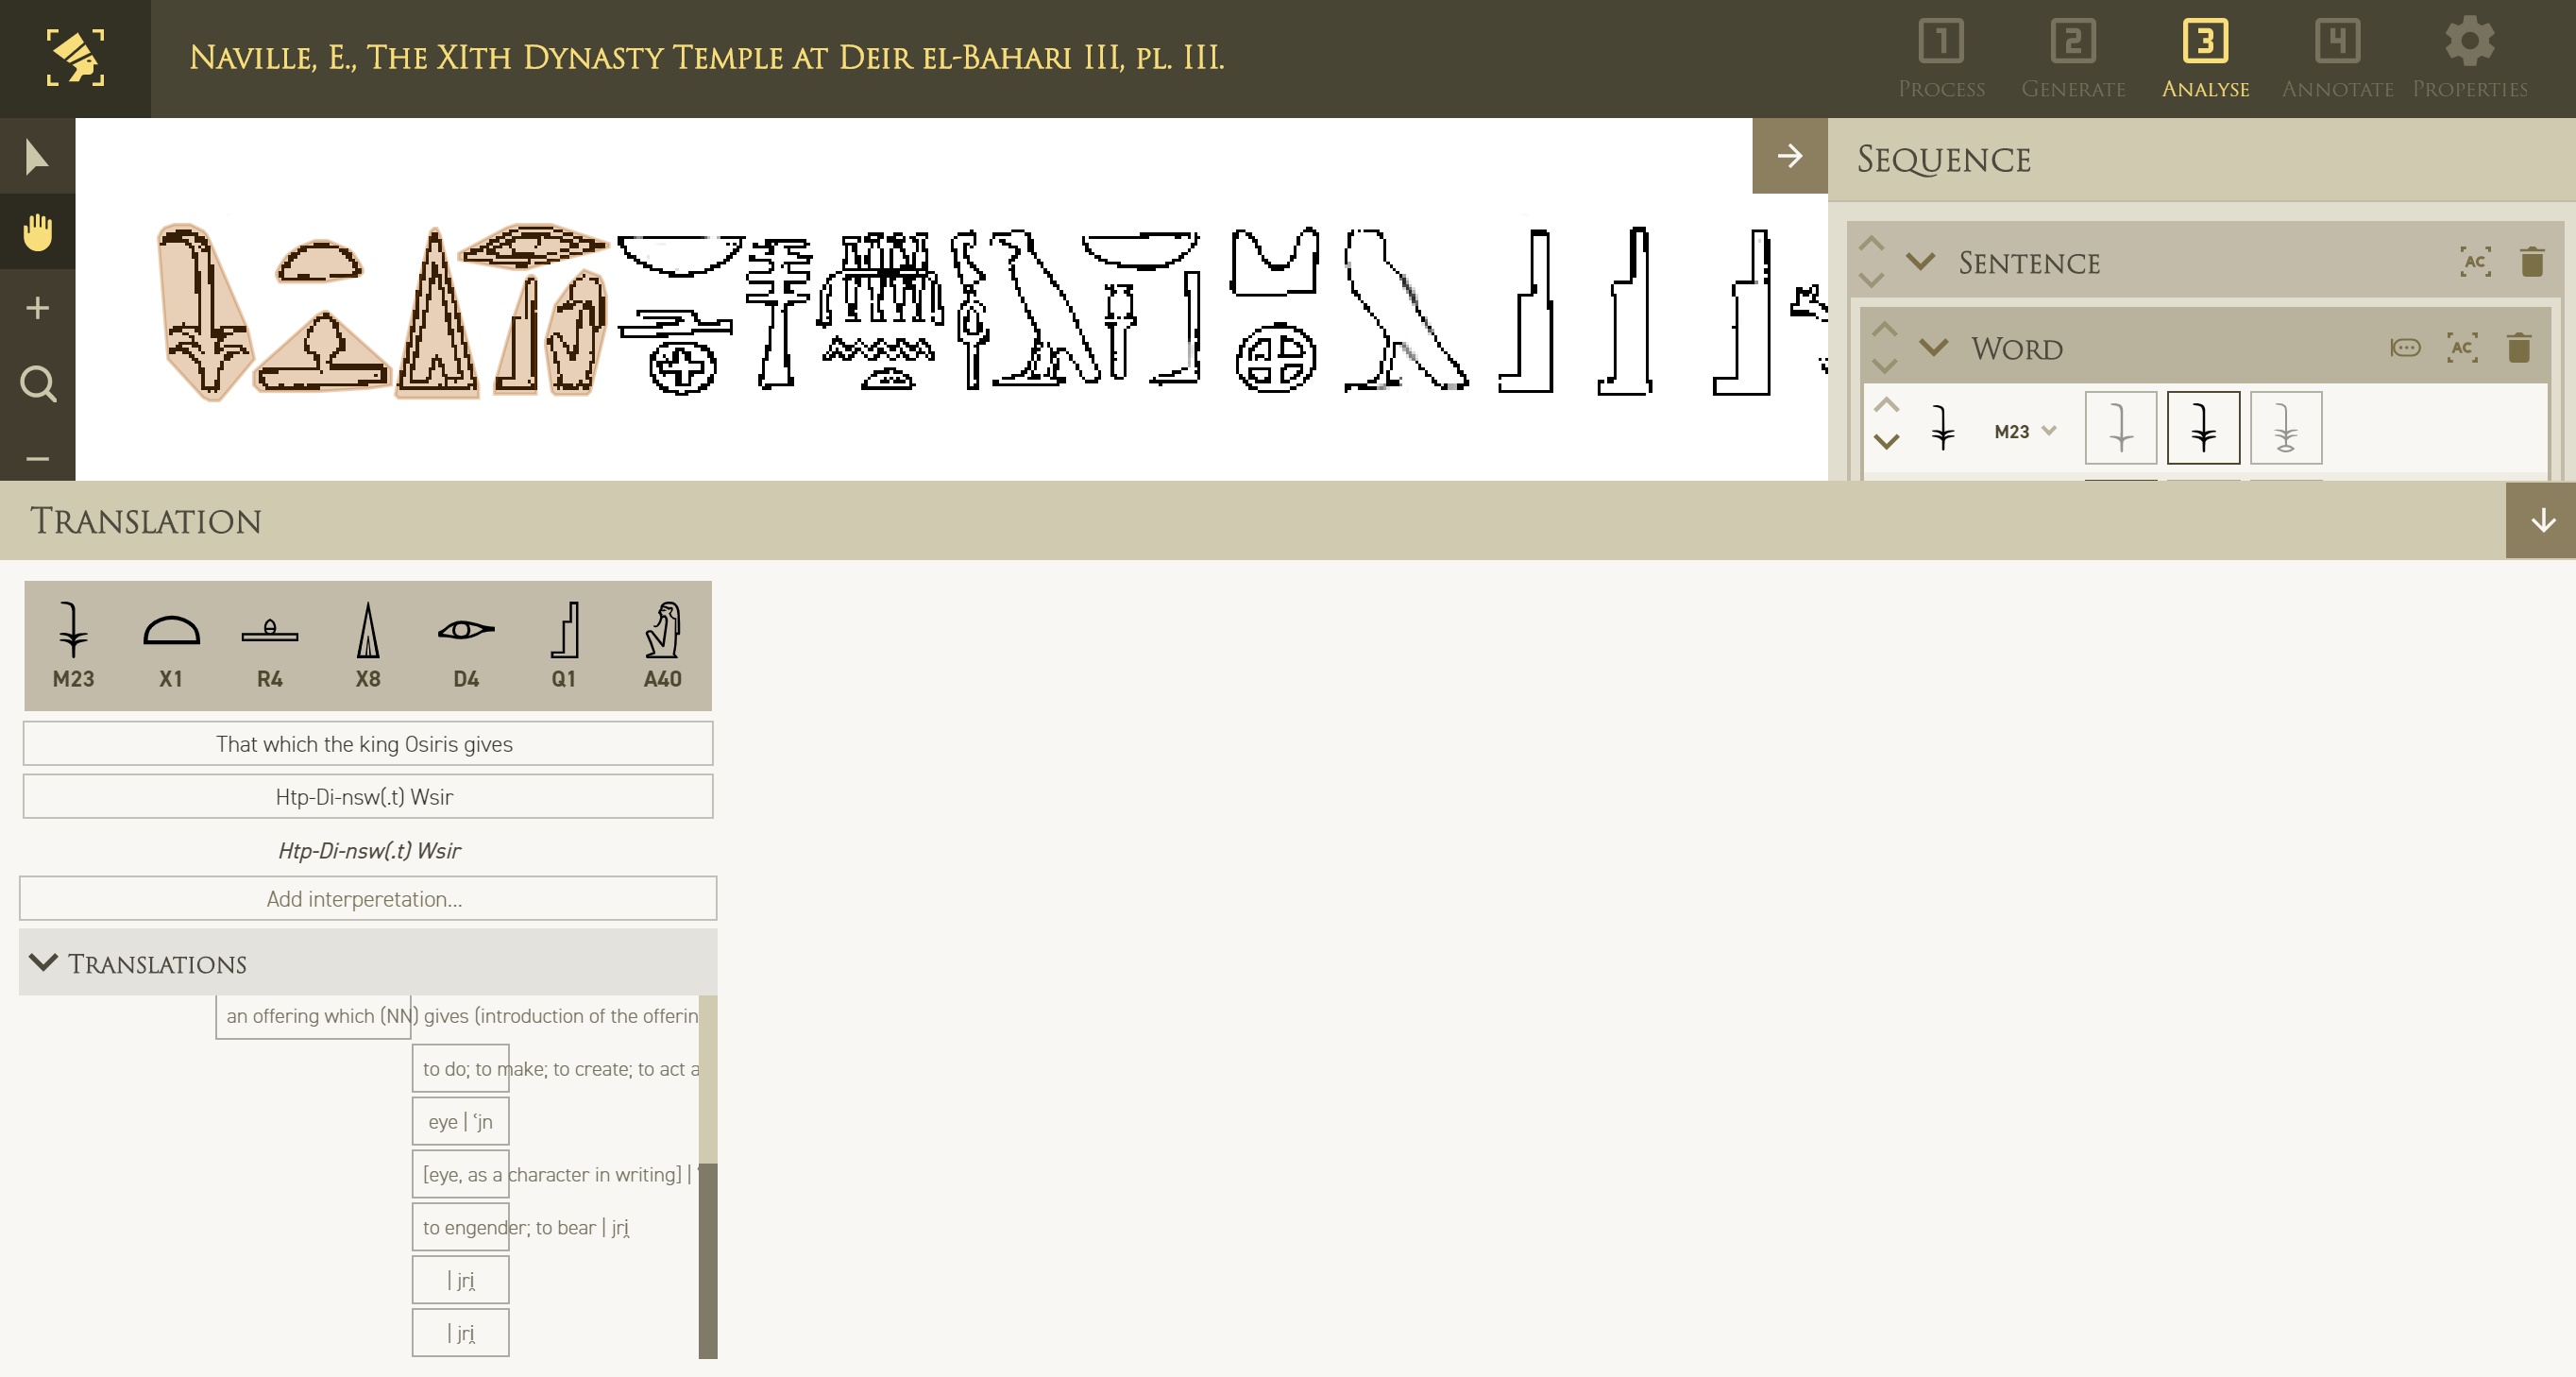
\includegraphics[width=1.0\textwidth]{hiero_16.PNG}
\break \noindent
The Auto-Translate tool seems to have quite accurately translated the phrase, and identified it as an offering formula, however, it appears that I can only read the full information, by either hovering the cursor over each line, or waiting until the translation section is dealing with a longer sentence (thus widening the Auto-Translation window). I have successfully produced a translation using The Hieroglyphics Initiative.
\newline \break \noindent
Step 5 achieved.
\newpage \break \noindent
\underline{Step 6}: Add some annotations to the project. Moving into the  ta, `4. Annotate,' I add a note to the phrase I have translated in the previous steps.
\newline \break

\includegraphics[width=1.0\textwidth]{hiero_17.PNG}
\break \noindent
I successfully add some comments using the Polygon tool to outline the grouping of glyphs I focused on during this exercise.
\newline \break
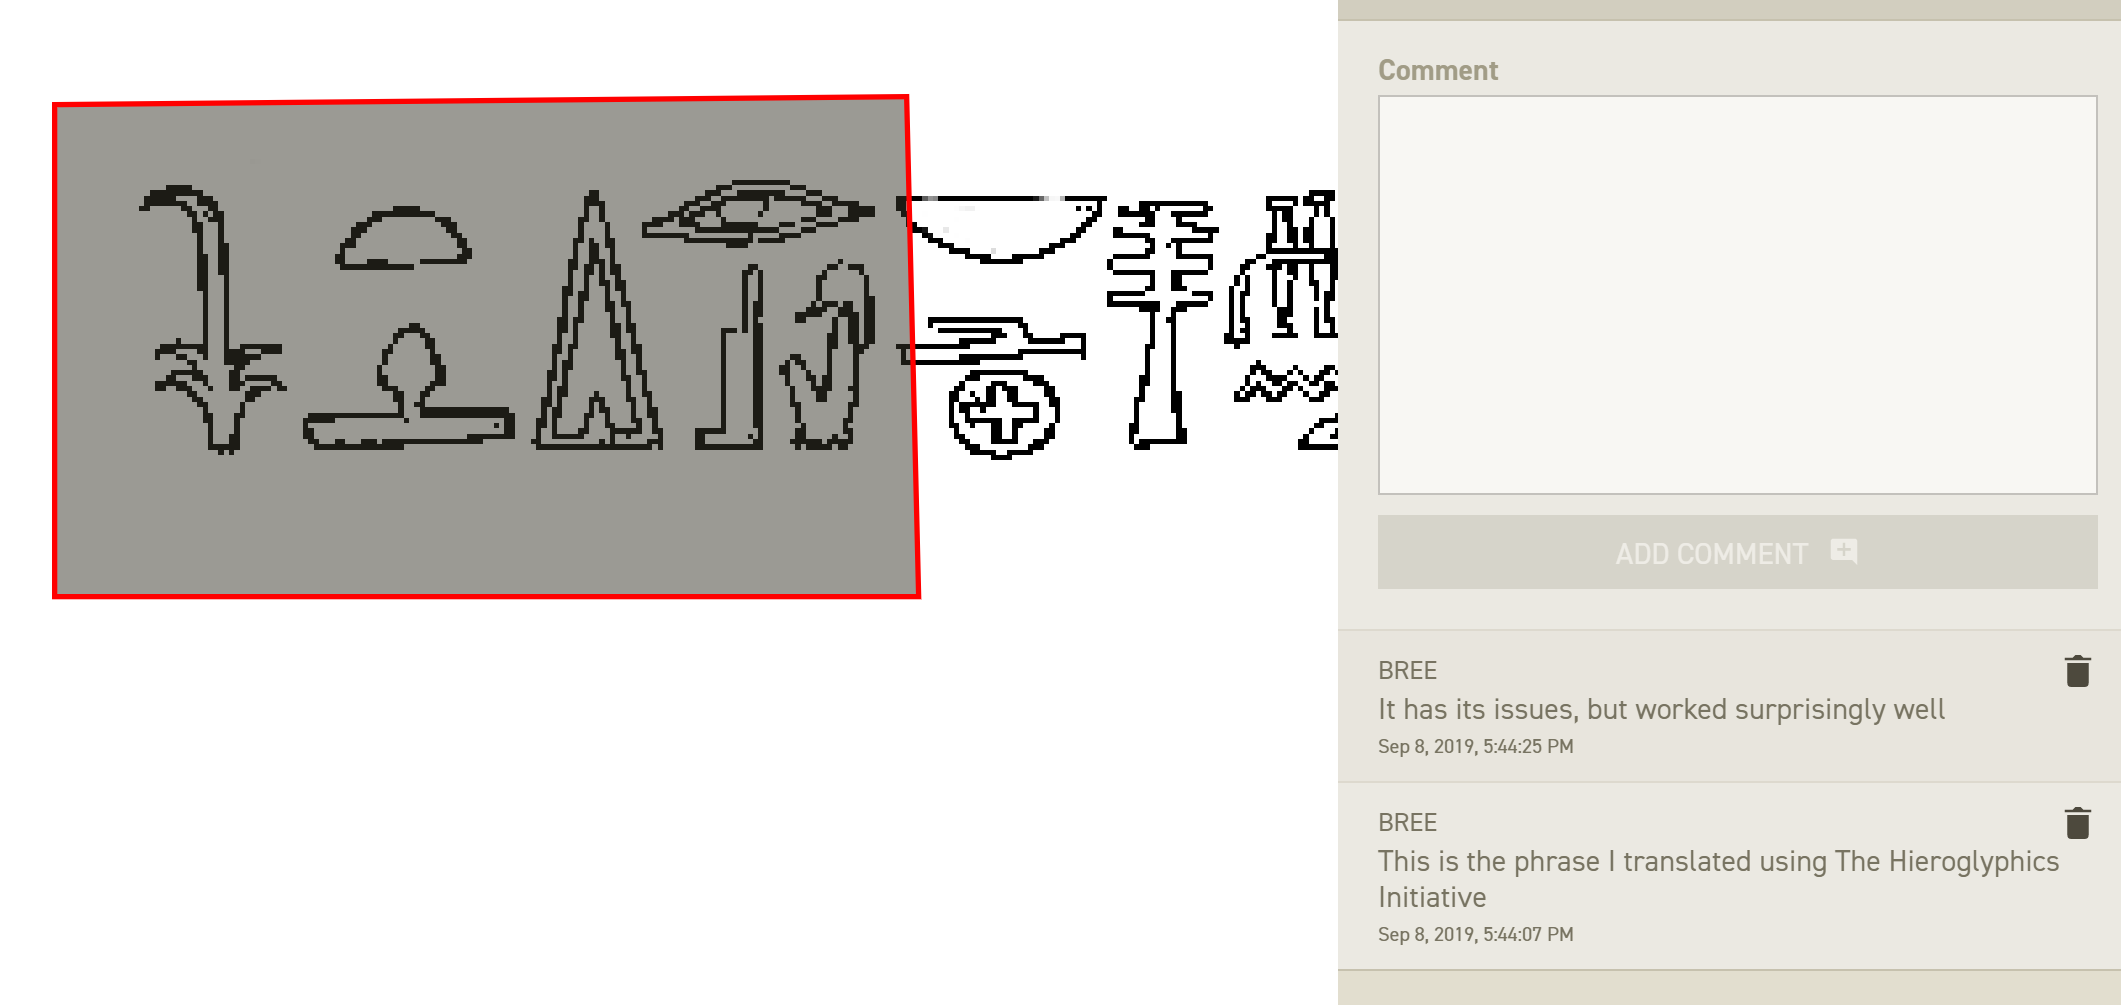
\includegraphics[width=1.0\textwidth]{hiero_18.PNG}
\break \noindent
Step 6 achieved.
\newline \break \noindent
\underline{Step 7}: Properties. Opening the final tab, `Properties,' I am presented with a number of options.
\newline \break

\includegraphics[width=1.0\textwidth]{hiero_20.PNG}
\break \noindent
I can add additional source files (I give this a go, and successfully upload a second PNG file to the project), I can rename the Project (but not the Author), I can delete source files (I delete the second PNG source file that I uploaded and it is removed without issue), and I can also delete the project. I do not try this option, as it will permanently delete my project. I can download the project as a WIP, which can be shared and worked on by others, or I can download my facsilime as an SVG (according to the documentation pdf). I follow both of these options and successfully download a YML file of the project as well as a PNG of the facsimile. I send these to Brian in an email to see if he can upload the YML file into his Workbench and work on it there. I can also view some information about the glyphs themselves:
\newline \break
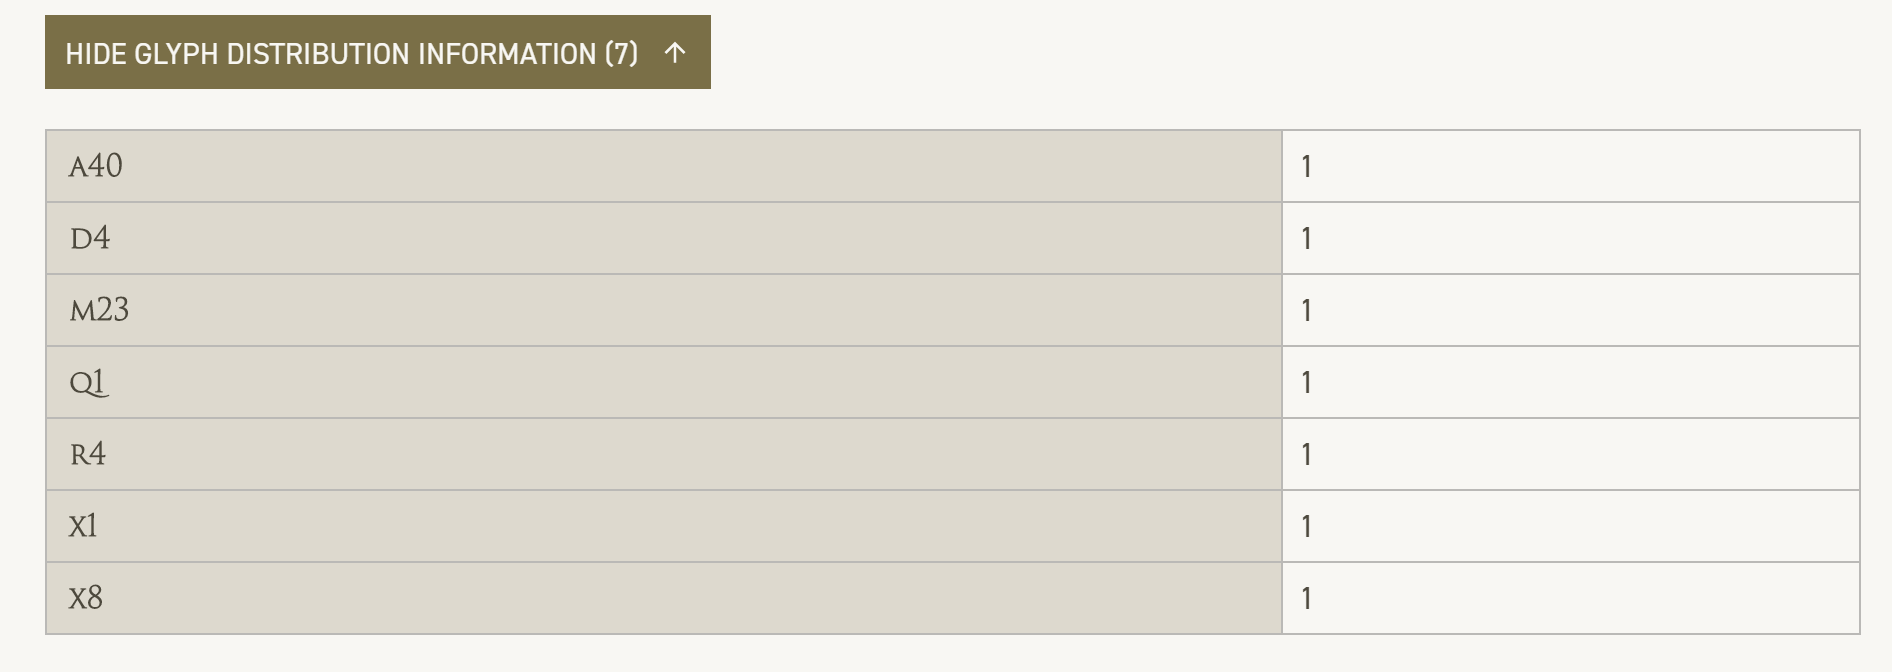
\includegraphics[width=1.0\textwidth]{hiero_19.PNG}
\break \noindent
I have successfully downloaded my project, saved it, and sent a copy of the YML file to Brian.
\newline \break \noindent
Step 7 achieved.
\paragraph{} ~\\\noindent
Based on my testing of The Hieroglyphics Initiative as a digital tool in the process of translating hieroglyphs (although incredibly rudimentary and brief), I believe I can attest to the functionality of the tool. It has a lot of limitations when it comes to uploading particular types of files, and not using specific web browsers, but this is not necessarily a huge problem. When it comes to streamlining the process of translation hieroglyphs within the field of Egyptology, it seems like having a quality threshold of images used (ie. limiting them to RAW) would be most beneficial, but would pose the question of where and how these were stored. Could a standardised system of data collection and storage be established, and how would access to repositories be managed? These are all considerations that will be explored at a later date. As for the present Elaboration exercise, The Hieroglyphics Initiative was able to be navigated without any major errors.

\end{document}